\documentclass[../main.tex]{subfiles}

\begin{document}

Firstly, there will be an endpoint handler handling all \textit{POST} requests at path \textit{/external-to-internal}. This endpoint handler will already accept only valid requests.

The endpoint will not contain business functionality, but will delegate the computation to the underlying service. Once the service responds with the result, endpoint simply returns the resulting DTO.

The above word description is visualized in Figure \ref{fig:translation-design}.

\begin{figure}
  \begin{center}
    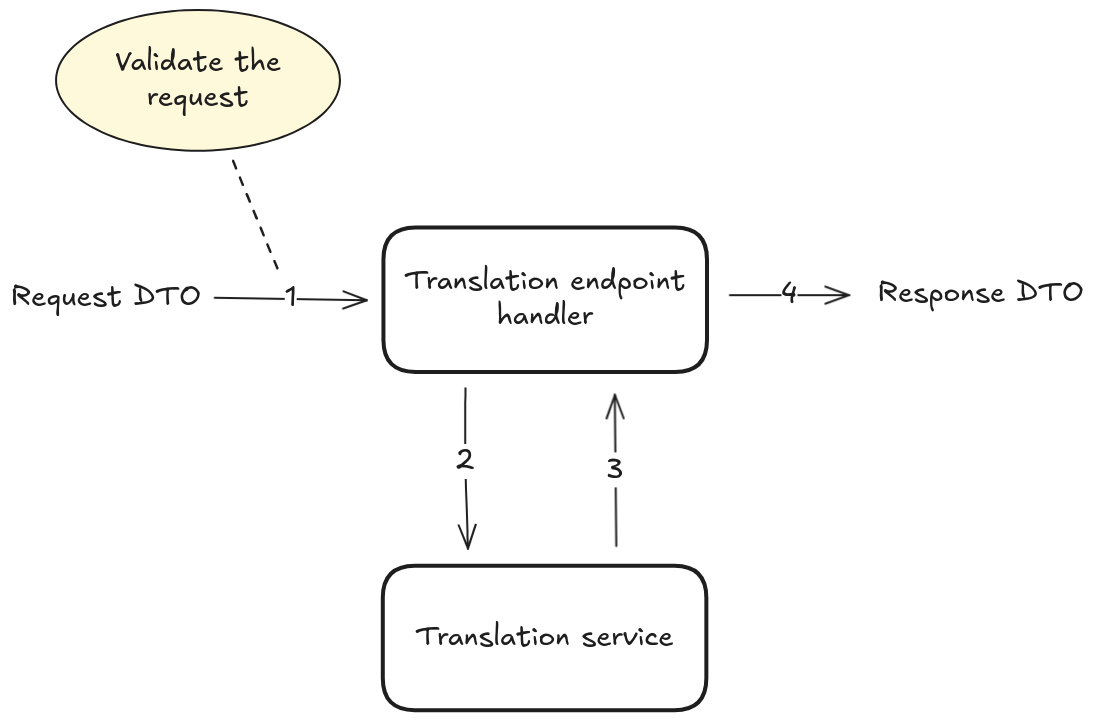
\includegraphics[width=0.8\textwidth]{images/translation-design.png}
  \end{center}
  \caption{Translation design}
  \label{fig:translation-design}
\end{figure}

\end{document}
